\documentclass[a4paper]{article}
\usepackage[T1]{fontenc}
\usepackage[utf8]{inputenc}
\usepackage{graphicx}

\title{EDA040 Android}
\date{}
\author{Oscar Olsson, 900311-0690\\ Tommy Olofsson, 900814-4553\\
	Erik Westrup, 901021-1192\\ Erik Jansson, 901202-4114}
\begin{document}
\maketitle

\section{Serversidan}
Servern stödjer bara en klient åt gången. Det finns en tråd (In) som lyssnar på inkommande data och blir blockerad av detta. Det finns en tråd som skriver till outputströmen till socketen. Båda dessa två använder ett objekt som implementerar nätverksprotokollet (ServerProtol) 

Det finns en tråd, ImageCapture, som blockeras vid bildhämtning vid från kameran. Bilder stoppas in i en monitor, ImageMonitor, där även rörelseavkänning påbilderna eventuellt görs. En bild åt gången sparas där.

Out-tråden kommer att blockeras i en metod getImage i ImageMonitorn och returnerar med en ny bild som eventuellt skrivs till outputströmen.

Vid initialt- och disconnected-tillstånd: en tråd, ConnectionSetup (main-tråd), väntar på anslutningar från en klient. När detta sker kommer den att skapa In \& out trådar. Övriga objekt återanvänds.

\newpage
\subsection{UML}
\begin{figure}[htb]
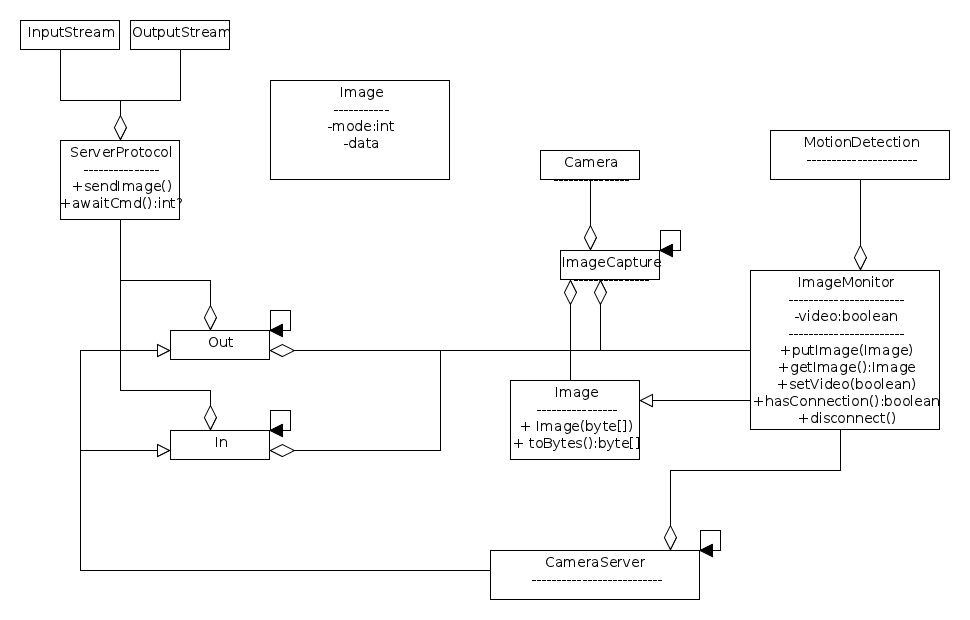
\includegraphics[scale=0.4]{uml_server.png}
\end{figure}

\section{Klientsidan}

Vår main-tråd är den vi kallar UI-tråden, som startas av Android-systemet, kommer att skapa programmets grafiska vyer. Dessa tar hand om alla användarinitiserade händelser. 

För varje ansluten kameraserver finns det en inputtråd som tar emot bilder. Bilderna stoppas in i en monitor som buffrar bilderna och tillhöran de data som timestamp.

Det finns en output-tråd som väntar på Commands i monitorn. När ett sådant finns tillgängligt skrivs detta på output-strömmen i ClientProtocol. Commands skapas av en Activity när användaren t.ex. klickar på en ev. "Idle mode"-knapp samt av monitorn när en bild har buffrats med "Video mode"-attribut.

ImageFetcher är en tråd som hämtar bilder från monitorn och ger dem till UI-tråden via en Activity. Detta är för att UI-tråden inte ska blockeras i monitorn. Monitorn innehåller all logik för att styra bildvisning i synkront läge. 

\newpage
\subsection{UML}
\begin{figure}[htb]
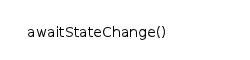
\includegraphics[scale=0.4]{uml_client.png}
\end{figure}

\end{document}
